\begin{figure}[h!]
	\centering
	
	
	
	\tikzset{every picture/.style={line width=0.75pt}} %set default line width to 0.75pt        
	
	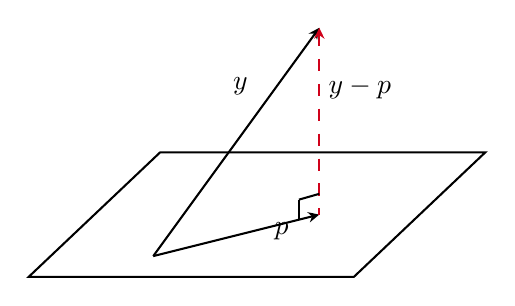
\begin{tikzpicture}[x=0.75pt,y=0.75pt,yscale=-1,xscale=1]
		%uncomment if require: \path (0,300); %set diagram left start at 0, and has height of 300
		
		%Shape: Parallelogram [id:dp4502347942292726] 
		\draw   (113.33,130) -- (270,130) -- (206.67,190) -- (50,190) -- cycle ;
		%Straight Lines [id:da3979852858777978] 
		\draw    (110,180) -- (187.09,160.73) ;
		\draw [shift={(190,160)}, rotate = 165.96] [fill={rgb, 255:red, 0; green, 0; blue, 0 }  ][line width=0.08]  [draw opacity=0] (5.36,-2.57) -- (0,0) -- (5.36,2.57) -- (3.56,0) -- cycle    ;
		%Straight Lines [id:da3930974235372434] 
		\draw    (110,180) -- (188.24,72.43) ;
		\draw [shift={(190,70)}, rotate = 126.03] [fill={rgb, 255:red, 0; green, 0; blue, 0 }  ][line width=0.08]  [draw opacity=0] (5.36,-2.57) -- (0,0) -- (5.36,2.57) -- (3.56,0) -- cycle    ;
		%Straight Lines [id:da43944712687476517] 
		\draw [color={rgb, 255:red, 208; green, 2; blue, 27 }  ,draw opacity=1 ] [dash pattern={on 4.5pt off 4.5pt}]  (190,73) -- (190,160) ;
		\draw [shift={(190,70)}, rotate = 90] [fill={rgb, 255:red, 208; green, 2; blue, 27 }  ,fill opacity=1 ][line width=0.08]  [draw opacity=0] (5.36,-2.57) -- (0,0) -- (5.36,2.57) -- (3.56,0) -- cycle    ;
		%Straight Lines [id:da4075325003962833] 
		\draw    (190,150) -- (180.2,152.8) ;
		%Straight Lines [id:da9654224371843569] 
		\draw    (180.2,152.8) -- (180.2,162.4) ;
		
		% Text Node
		\draw (167,162.4) node [anchor=north west][inner sep=0.75pt]    {$p$};
		% Text Node
		\draw (147,92.4) node [anchor=north west][inner sep=0.75pt]    {$y$};
		% Text Node
		\draw (193,92.4) node [anchor=north west][inner sep=0.75pt]    {$y-p$};
		
		
	\end{tikzpicture}
\end{figure}